\section{Question 1 - \textit{word count: 946}}



In order to calculate the energy storage capacity that Scotland requires to satisfy its electricity demand at all times with renewable generation, the following needs to be done beforehand:
\begin{itemize}
	\item Determine Scotland's current typical electricity demand
	\item Upscale the current generation mix for renewable technologies
	\item Calculate the necessary power rating for the energy storage
\end{itemize}



%%% SUBSECTION %%%

\subsection{Typical electricity demand}

The Department for Business, Energy {\&} Industrial Strategy (BEIS) of the UK Government publishes electricity generation and supply statistics on a quarterly basis \citep{BEIS2018ElecUK}.
Table~\ref{tbl:elec_demand} presents the most up-to-date figures for Scotland.
England is a regular importer of electricity from Scotland \citep{BEIS2018EnergyTrends}.
Northern Ireland usually imports electricity from Scotland but was a net exporter to Scotland for the first time in 2016, which continued in 2017 \citep{BEIS2018EnergyTrends}.
Scotland's annual demand is calculated by subtracting the exported electricity from and adding the imported electricity to its total generation.
This gives Scotland a current typical electricity demand of 35,810~GWh.

% Please add the following required packages to your document preamble:
% \usepackage{booktabs}
\begin{table}[htbp]
	\caption{Generation, exports, imports and demand of electricity in Scotland in 2017 \citep{BEIS2018ElecUK}.}
	\label{tbl:elec_demand}
	\centering
	\begin{tabular}{@{}lr@{}}
		\toprule
		Electricity in Scotland 2017 & GWh \\ \midrule
		Total generated & 48,678 \\
		Electricity exported to England & -13,013 \\
		Electricity imported from Northern Ireland & 145 \\ \midrule
		Demand (sum of above) & 35,810 \\ \bottomrule
	\end{tabular}
\end{table}



%%% SUBSECTION %%%

\subsection{Upscale of renewable generation mix}

Tables~\ref{tbl:installed_cap}, \ref{tbl:RE_gen} and \ref{tbl:days} respectively present the installed capacity of renewable technologies in Scotland, the renewable energy (RE) generation in Scotland and the number of days per year from 2012 or 2013 to 2017.
Equation~\ref{eq:CF} represents the annual capacity factor (CF), i.e. the ratio of annual energy yield over the maximum possible annual energy yield.
The capacity factors for Scotland's renewable technologies were calculated per year by inputting the data in the aforementioned tables in Equation~\ref{eq:CF}.
Equation~\ref{eq:CF_example} demonstrates this with the calculation of the capacity factor for onshore wind energy in 2013.
The capacity factors and their averages are presented in Table~\ref{tbl:CFs}.

% Please add the following required packages to your document preamble:
% \usepackage{booktabs}
\begin{table}[H]
	\caption{Cumulative installed capacity of renewable technologies in Scotland from 2012 to 2017 \citep{BEIS2018REs}.}
	\label{tbl:installed_cap}
	\centering
	\begin{tabular}{@{}lrrrrrr@{}}
		\toprule
		Cumulative installed capacity (MW) & 2012 & 2013 & 2014 & 2015 & 2016 & 2017 \\ \midrule
		Onshore Wind & 3,765 & 4,589 & 5,079 & 5,398 & 6,327 & 7,389 \\
		Offshore Wind & 190 & 190 & 197 & 187 & 187 & 246 \\
		Shoreline wave / tidal & 7 & 7 & 7 & 8 & 13 & 18 \\
		Solar PV & 95 & 133 & 175 & 264 & 326 & 323 \\
		Small scale Hydro & 158 & 171 & 189 & 232 & 290 & 313 \\
		Large scale Hydro & 1,339 & 1,339 & 1,339 & 1,339 & 1,339 & 1,341 \\
		Landfill gas & 115 & 115 & 116 & 116 & 116 & 116 \\
		Sewage sludge digestion & 9 & 7 & 7 & 7 & 7 & 7 \\
		Other biomass & 138 & 150 & 230 & 236 & 259 & 295 \\ \bottomrule
	\end{tabular}
\end{table}

% Please add the following required packages to your document preamble:
% \usepackage{booktabs}
\begin{table}[H]
	\caption{RE generation in Scotland from 2013 to 2017 \citep{BEIS2018REs}.}
	\label{tbl:RE_gen}
	\centering
	\begin{tabular}{@{}lrrrrr@{}}
		\toprule
		RE Generation (GWh) & 2013 & 2014 & 2015 & 2016 & 2017 \\ \midrule
		Onshore Wind & 10,563 & 11,130 & 13,340 & 11,954 & 16,448 \\
		Offshore Wind & 587 & 569 & 539 & 502 & 616 \\
		Shoreline wave / tidal & 1 & 2 & 2 & 0 & 4 \\
		Solar PV & 96 & 143 & 186 & 276 & 290 \\
		Hydro & 4,369 & 5,484 & 5,814 & 5,149 & 5,356 \\
		Landfill gas & 563 & 533 & 503 & 493 & 445 \\
		Sewage sludge digestion & 31 & 28 & 26 & 32 & 36 \\
		Other biomass (inc. co-firing) & 778 & 1,155 & 1,334 & 1,374 & 1,971 \\ \bottomrule
	\end{tabular}
\end{table}

% Please add the following required packages to your document preamble:
% \usepackage{booktabs}
\begin{table}[H]
	\caption{Number of days in the years from 2013 to 2017 \citep{BEIS2018REs}.}
	\label{tbl:days}
	\centering
	\begin{tabular}{@{}lrrrrr@{}}
		\toprule
		Year & 2013 & 2014 & 2015 & 2016 & 2017 \\ \midrule
		Days & 365 & 365 & 365 & 366 & 365 \\ \bottomrule
	\end{tabular}
\end{table}

\input{tables/CFs}

	\begin{equation}\label{eq:CF}
		\begin{split}
			CF & = \frac{annual\;energy\;yield\;[MWh]}{maximum\;possible\;energy\;yield\;[MWh]} \\
			& \\
			& = \frac{generation\;[MWh]}{average\;capacity\;[MW] \times hours\;in\;the\;year\;[h]}
		\end{split}
	\end{equation}

	\begin{equation}\label{eq:CF_example}
		\begin{split}
			CF_{onshore\;wind,\;2013} & = \frac{2013\;generation\;[GWh] \times 1000}{\frac{2012\;capacity\;+\;2013\;capacity}{2}\;[MW] \times 24\;[h] \times days\;in\;2013} \\
			& \\
			& = \frac{10,563\;[GWh] \times 1000}{\frac{3,765\;+\;4,589}{2}\;[MW] \times 24\;[h] \times 365} = \frac{10,563,000\;[MWh]}{4,177\;[MW] \times 8,760\;[h]} \\
			& \\
			& = 29\%
		\end{split}
	\end{equation}

Using the average capacity factors and the cumulative installed capacity of renewable technologies from 2017, the typical RE generation in Scotland can be calculated (see Table~\ref{tbl:upscale}).
This is calculated by re-arranging Equation~\ref{eq:CF} for generation.
It was found that, currently, Scotland's RE generation typically meets 73.4\% of its electricity demand of 35,810~GWh.
By upscaling the 2017 cumulative installed capacity by 36.4\%, the subsequent RE generation can meet 100\% of Scotland's demand.

% Please add the following required packages to your document preamble:
% \usepackage{booktabs}
\begin{table}[htbp]
	\caption{.}
	\label{tbl:upscale}
	\centering
	\begin{tabu} to \textwidth {@{}lX[r]X[r]X[r]lX[r]X[r]@{}}
		\toprule
		\multicolumn{1}{r}{} & \multicolumn{1}{r}{\textbf{2012-2017}} & \multicolumn{1}{r}{\textbf{2017}} & \multicolumn{1}{r}{\textbf{Typical}} &  & \multicolumn{2}{r}{\textbf{Scenario: Scale up 36.4\%}} \\
		& Average Capacity Factors & Cumulative Installed Capacity (MW) & RE Generation (GWh) &  & Cumulative Installed Capacity (MW) & RE Generation (GWh) \\ \midrule
		Onshore Wind & 27\% & 7,389 & 17,452 &  & 10,079 & 23,805 \\
		Offshore Wind & 33\% & 246 & 707 &  & 336 & 964 \\
		Shoreline wave / tidal & 2\% & 18 & 3 &  & 25 & 5 \\
		Solar PV & 10\% & 323 & 287 &  & 441 & 392 \\
		Small scale Hydro & 38\% & 313 & 1,047 &  & 427 & 1,429 \\
		Large scale Hydro & 38\% & 1,341 & 4,487 &  & 1,829 & 6,121 \\
		Landfill gas & 50\% & 116 & 508 &  & 158 & 693 \\
		Sewage sludge digestion & 48\% & 7 & 29 &  & 10 & 40 \\
		Other biomass & 68\% & 295 & 1,762 &  & 402 & 2,403 \\ \midrule
		Total &  & 10,049 & 26,283 &  & 13,705 & 35,851 \\ \midrule
		\multicolumn{3}{l}{Percentage of typical demand (35,810 GWh)} & 73.4\% &  &  & 100.1\% \\ \bottomrule
	\end{tabu}
\end{table}



%%% SUBSECTION %%%

\subsection{Power rating}

\hl{intro}



\subsubsection{Peak power demand}

Since Scotland's peak power demand proved challenging to find, it was deduced from the overall UK demand.
In 2017, the UK's peak power demand was 52.279~GW \citep{BEIS2018PeakDemand} and Scotland's population accounted for 8.2\% of the total UK population \citep{OfficeforNationalStatistics2018}.
Therefore, it can be assumed that Scotland's peak power demand is 8.2\% of the UK demand, i.e. 4.29~GW.

However, this demand does not account for losses in transmission etc.
The losses were found by subtracting Scotland's total electricity consumption in 2017 of 30,590~GWh \citep{BEIS2018ElecUK} from Scotland's annual electricity demand of 35,810~GWh.
The losses, 5,220~GWh, represent 15\% of the annual energy demand.
Therefore, Scotland's peak power demand was scaled up by 15\% to account for losses; this results in 4.91~GW.



\subsubsection{Base load}

For the base load includes all dispatchable loads that can be turned on and off at any given time.
This consists of 116~MW of landfill gas, 7~MW of sewage sludge digestion, and 295~MW of other biomass (see Table~\ref{tbl:installed_cap}).
Large scale hydro can also be considered dispatchable, but its load will depend on precipitation which varies largely by season.
Figure~\ref{fig:hydro_distribution} shows that hydro in the UK has an average capacity factor of 50\% in the winter; this is assumed to coincide with Scotland's peak electricity demand due to the increased need for lighting and heating\footnote{However, it should be noted that there might be discrepancies between hydro's capacity factors in the UK and Scotland.}.
Therefore, the base load also consists of 50\% of the installed capacity for large scale hydro, i.e. 50\% of 1,341~MW which equals 670.5~MW (see Table~\ref{tbl:installed_cap}).
In total, the base load amounts to 1.48~GW.

\begin{figure}[htbp]
	\centering
	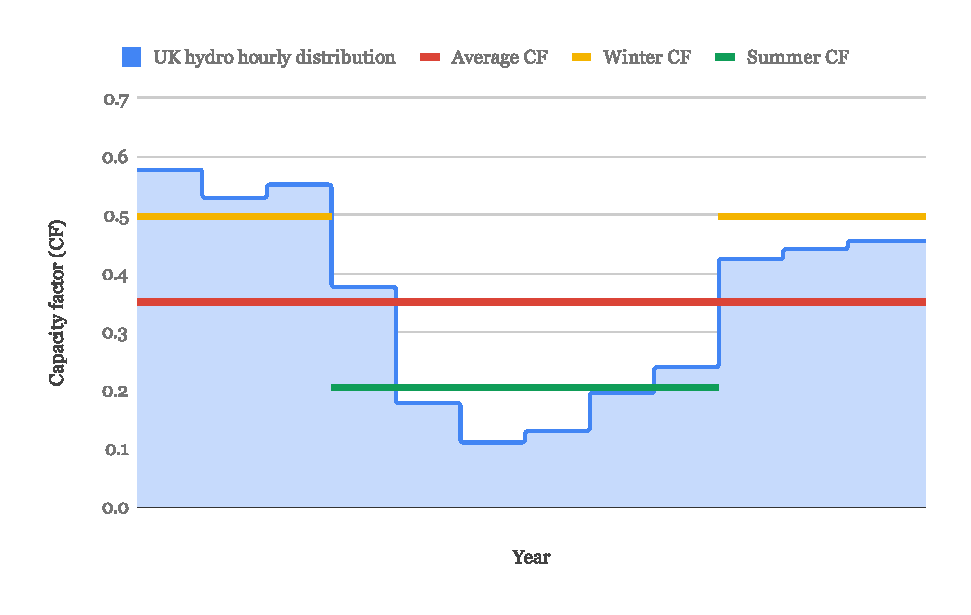
\includegraphics[width=\textwidth]{figures/Hydro_distribution.eps}
	\rule{\textwidth}{0.5pt} % use line???
	\caption{The capacity factors for UK's hydro throughout the year, including the average annual, average winter and average summer capacity factors. This chart is based on ``AA hydro uk hourly.txt" hourly distribution data from EnergyPLAN's UK 2020 Model \citep{EnergyPLAN_UK2020}.}
	\label{fig:hydro_distribution}
\end{figure}


\subsubsection{Necessary power rating}

The necessary energy storage power rating to meet Scotland's peak demand can then simply be calculated as the difference between its peak power demand (including losses) and base load, i.e. $4.91~GW - 1.48~GW = 3.43~GW$.



%%% SUBSECTION %%%

\subsection{Necessary energy storage capacity}

In a study done by Siemens, it was found that to have all electricity in Europe supplied by renewables, ``both reinforcement of interconnection lines and EES [electrical energy storage] capacity of between 2\% and 8\% of the annual total demand is necessary" \citep[p.~69]{IEC2011}.
Considering the worst case scenario for Scotland, it is assumed 8\% of its demand is needed in annual storage, i.e. 2,865~GWh.
However, this annual storage demand risks being too low since Scotland is independent from interconnects in this case study.

The following is an alternative way to calculate Scotland's required energy storage capacity, inspired by Mearns \citep{Mearns2018}.
Figure~\ref{fig:winter_demand} shows that Scotland's mean winter demand is 2.91~GW.
Assuming the base load meets 1.48~GW of this, Scotland's energy storage is required to meet the remaining demand, i.e. 1.43~GW.
Scotland's energy storage capacity (in GWh) depends on the time period energy storage is considered necessary for.
Considering that wind is Scotland's largest renewable source of energy (see Table~\ref{tbl:RE_gen}), and the most variable, the time period can be based on typical periods of low wind generation.
In the UK's wind output for 2017 \citep{GridWatchnd}, the longest time period of consistently low wind generation was found to be three days (the criterion for low output was arbitrarily chosen to be 10\% or less of the maximum output)\footnote{This data has just been used for indication. It should be noted that this data regards the whole of the UK as opposed to just Scotland, and that it covers just a year as opposed to a ten year period, which is generally considered to be representative of the local wind climate \citep[p.~15]{Boehme2006}.}.
Hence, Scotland should have at least three days' worth of energy storage capacity, i.e. $1.43~GW \times 24~hours \times 3~days = 103~GWh$.
However, one may want to design for more storage in case of longer periods of low wind generation.
Storage capacity options of between three and seven days are presented in Figure~\ref{fig:storage_options}.
The annual energy storage demand calculated using this same method, i.e. multiplied by 365~days, is 12,527~GWh which represents 35\% of Scotland's annual demand.
This is about four times greater than the 8\% capacity calculated earlier.
It is possible that in the Siemens case study, interconnects are expected to supply between 27\% and 33\% of the annual energy demand alongside the energy storage of 2\%--8\%.

\hl{input figures/winter demand}

\begin{figure}[htbp]
	\centering
	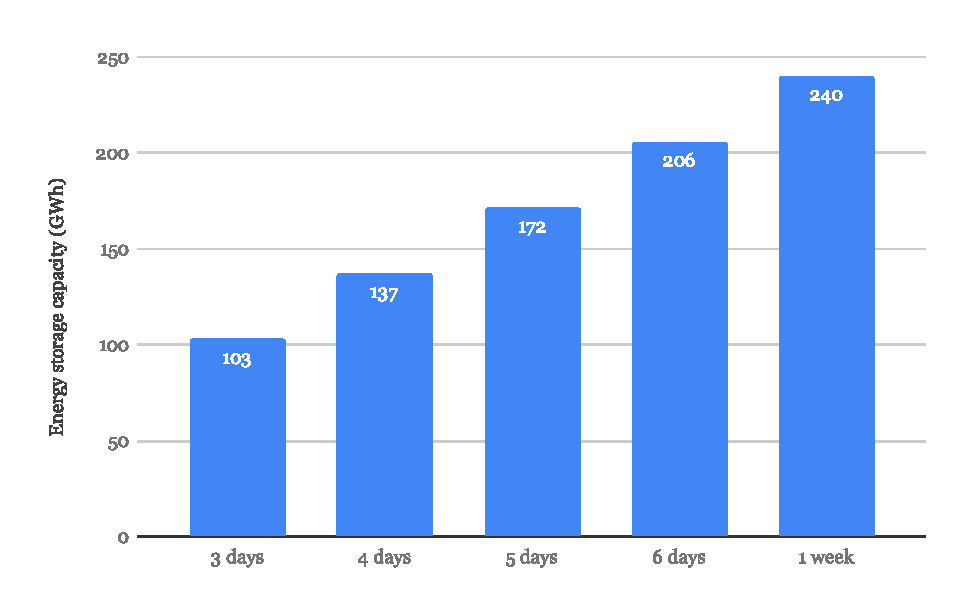
\includegraphics[width=.7\textwidth]{figures/storage_options.eps}
	\rule{\textwidth}{0.5pt} % use line???
	\caption{Energy storage capacity options for Scotland in function of time periods of low wind generation.}
	\label{fig:storage_options}
\end{figure}

\hl{power to energy ratio/ marathon vs sprinter battery modes?}

\hl{long storage durations: ``Owing to the small evaporation
and penetration, the storage period of PHS can be varied
from typically hours to days and even years."}
Suitable storage duration: hours - months.
 \citep{Chen2009}

\begin{comment}
\textbf{Power-to-energy ratio (P/E ratio)}

``If the battery system will be used primarily to provide frequency regulation, the battery system needs to charge and discharge many times over short durations of time. A system used in this type of scenario will be designed with a higher power rating. If a battery system will be used primarily to provide peak-shifting or must provide backup power in case of a grid outage, the battery needs to be able to discharge over a longer period (e.g., 2 – 5 hours) and is designed with a higher energy rating."
\url{https://www.nrel.gov/state-local-tribal/blog/posts/batteries-101-series-how-to-talk-about-batteries-and-power-to-energy-ratios.html}

C.f. ``"Marathon" and "sprinter" metrics"
\url{https://www.greentechmedia.com/articles/read/comparing-energy-storage-its-not-that-simple#gs.3osuww}

``Concluding Thoughts
The optimum specifications for a PHS scheme in Scotland used to store surplus wind power for use during calm periods should have a power / stored energy ratio ~ 0.006. Given the storage size of Coire Glas = 30 GWh the power rating should ideally be ~ 180 MW and not the massive 1500 MW now proposed for the site. The 180 MW power rating would drain the reservoir in 7 days of continuous name plate capacity use. The facility would now be used for 7 out of 21 days (A+B+C), i.e. the equivalent of 1 day in 3 which is the closest we have got to every day, the norm for making PHS profitable. The catch now, however, is that the puny beast has now become totally limp with a power rating of only 180 MW – it can never ever make money."
\url{http://euanmearns.com/coire-glas-the-raging-best-of-pumped-hydro-storage/}
\end{comment}